\documentclass[12pt, a4paper]{report}

% Packages :

\usepackage[french]{babel}
\usepackage[utf8]{inputenc}
\usepackage[T1]{fontenc}
\usepackage[pdftex, pdfauthor={Bacomathiques}]{hyperref}
\usepackage{sectsty}
\usepackage[explicit]{titlesec}
\usepackage{xcolor}
\usepackage{amsmath}
\usepackage{amssymb}
\usepackage{amsthm}
\usepackage{fourier}
\usepackage{titlesec}
\usepackage{fancyhdr}
\usepackage{catchfilebetweentags}
\usepackage[french, capitalise, noabbrev]{cleveref}
\usepackage[fit, breakall]{truncate}
\usepackage[margin=3cm]{geometry}
\usepackage{tocloft}
\usepackage{tikz}
\usepackage{tocloft}
\usepackage{microtype}
\usepackage{listings}
\usepackage{tabularx}
\usepackage{calc}
\usepackage[export]{adjustbox}
\usepackage[most]{tcolorbox}
\usepackage{standalone}
\usepackage{xlop}
\usepackage{etoolbox}
\usepackage{environ}

\usetikzlibrary{arrows.meta}
\usetikzlibrary{trees}

% Paramètres :

\author{Bacomathiques}
\definecolor{graphe}{HTML}{93c9ff}
\setcounter{MaxMatrixCols}{12}
\setlength{\parindent}{0pt}
\setlength{\fboxsep}{0pt}
%\pdfsuppresswarningpagegroup=1

% Code :

\lstdefinestyle{style}{
	backgroundcolor=\color{white},
	commentstyle=\em\color[HTML]{999988},
	keywordstyle=\bfseries,
	identifierstyle=\normalfont,
	stringstyle=\color[rgb]{0.87, 0.07, 0.27},
	basicstyle=\ttfamily\color{black},
	breakatwhitespace=false,
	breaklines=true,
	captionpos=b,
	keepspaces=true,
	numbers=left,
	numbersep=5pt,
	showspaces=false,
	showstringspaces=false,
	showtabs=false,
	tabsize=2,
	numbers=none
}

\lstset{style=style}
\lstset{
	literate=
	{á}{{\'a}}1
	{à}{{\`a}}1
	{ã}{{\~a}}1
	{é}{{\'e}}1
	{ê}{{\^e}}1
	{í}{{\'i}}1
	{ó}{{\'o}}1
	{õ}{{\~o}}1
	{ú}{{\'u}}1
	{ü}{{\"u}}1
	{ç}{{\c{c}}}1
}

\lstset{
	framextopmargin=10pt,
	framexrightmargin=10pt,
	framexbottommargin=10pt,
	framexleftmargin=10pt,
	xleftmargin=10pt,
	xrightmargin=10pt,
}

% Couleurs :

\definecolor{title}{HTML}{912c21}
\definecolor{section}{HTML}{1c567d}
\definecolor{subsection}{HTML}{2980b9}

\definecolor{rule}{HTML}{c4c4c4}

\definecolor{formula}{HTML}{ebf3fb}
\definecolor{formula-left}{HTML}{3583d6}

\definecolor{tip}{HTML}{dcf3d8}
\definecolor{tip-left}{HTML}{26a65b}

\definecolor{demonstration}{HTML}{fff8de}
\definecolor{demonstration-left}{HTML}{f1c40f}

\definecolor{exercise}{HTML}{e0f2f1}
\definecolor{exercise-left}{HTML}{009688}

\definecolor{correction}{HTML}{e0f7fa}
\definecolor{correction-left}{HTML}{00bcd4}

\definecolor{toc}{HTML}{fceae9}
\definecolor{toc-left}{HTML}{e74c3c}
\definecolor{toc-dark}{HTML}{87281f}

% Titres :

\renewcommand{\thesection}{\Roman{section} - }
\renewcommand{\thesubsection}{\arabic{subsection}. }

\newcommand{\sectionstyle}{\normalfont\LARGE\bfseries\color{section}}
\titleformat{\section}{\sectionstyle}{\thesection #1}{0pt}{}
\titleformat{name=\section, numberless}{\sectionstyle}{#1}{0pt}{}

\newcommand{\subsectionstyle}{\normalfont\Large\bfseries\color{subsection}}
\titleformat{\subsection}{\subsectionstyle}{\thesubsection #1}{0pt}{}
\titleformat{name=\subsection, numberless}{\subsectionstyle}{#1}{0pt}{}

\titlelabel{\thetitle\ }

% Table des matières :

\addto\captionsfrench{\renewcommand\contentsname{}}
\renewcommand{\cftsecpagefont}{\color{toc-dark}}
\renewcommand{\cftsubsecpagefont}{\color{toc-dark}}
\renewcommand{\cftsecleader}{\cftdotfill{\cftdotsep}}
\renewcommand{\cftsecfont}{\bfseries}
\renewcommand{\cftsecpagefont}{\bfseries\color{toc-dark}}
\setlength{\cftbeforetoctitleskip}{0pt}
\setlength{\cftaftertoctitleskip}{0pt}
\setlength{\cftsecindent}{0pt}
\setlength{\cftsubsecindent}{20pt}
\setlength{\cftsubsecnumwidth}{20pt}

% Commandes :

\newcommand{\newpar}{\\[\medskipamount]}
\newcommand{\lesson}[3]{%
	\newcommand{\level}{#1}%
	\newcommand{\id}{#2}%
	\hypersetup{pdftitle={#3}}
	\begin{center}%
		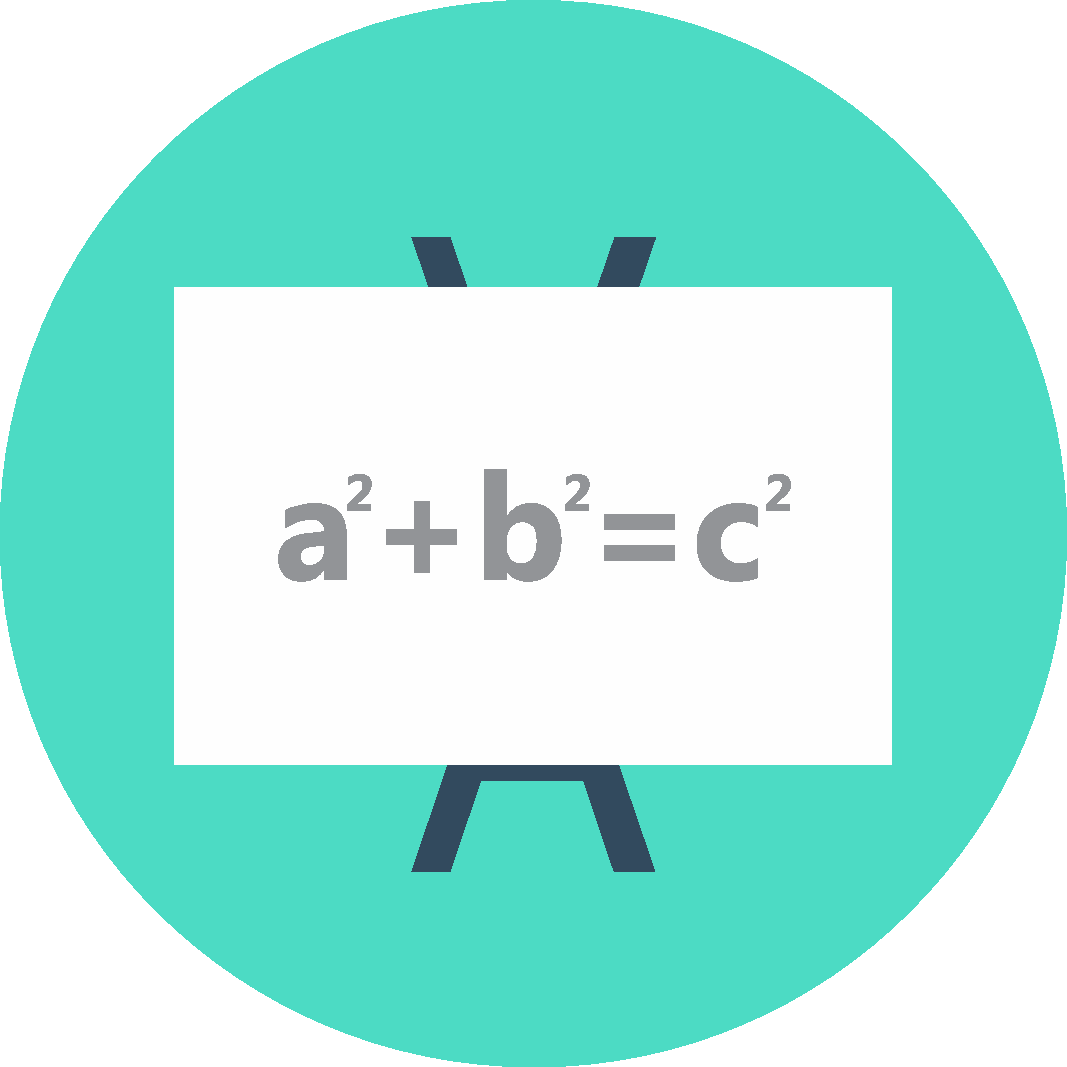
\includegraphics[width=150px]{\imagespath/bacomathiques}%
		
		\vspace{30pt}%
		{\Huge\color{title} #3}%
		
		\vspace{10pt}%
		{Bacomathiques --- \href{https://bacomathiqu.es/cours/#1/#2}{\color{section} https://bacomathiqu.es}}%
		
		\vspace{20pt}%
	\end{center}%
	\begin{toc}
		\tableofcontents%
	\end{toc}
	\thispagestyle{empty}%
	\newpage%
	\setcounter{page}{1}%
}
\newcommand{\imagespath}{../../images}
\newcommand{\lessonimagespath}{\imagespath/lessons/\level/\id/}
\newcommand{\includelatexpicture}[2][\textwidth - 100pt]{%
	\begin{center}%
		\resizebox{#1}{!}{%
			\input{\lessonimagespath#2}%
		}%
	\end{center}%
	\medskip%
}
\newcommand{\includeimage}[1]{%
	\begin{center}%
		\includegraphics{\lessonimagespath#1}%
	\end{center}%
	\medskip%
}
\newcommand{\includerepresentation}[1]{%
	\begin{center}%
		\setlength{\fboxrule}{0.5pt}%
		\href{https://www.geogebra.org/m/#1}{\includegraphics[width=\textwidth-1pt,fbox]{\lessonimagespath#1}}%
	\end{center}%
}
\newcommand{\floor}[1]{\lfloor #1 \rfloor}

\makeatletter
\newcommand\inputcontent{\@ifstar{\inputcontent@star}{\inputcontent@nostar}}
\newcommand{\inputcontent@star}[1]{%
	\ExecuteMetaData[#1]{content}%
}
\newcommand{\inputcontent@nostar}[1]{%
	\newpage%
	\inputcontent@star{#1}%
}
\makeatother

\let\oldsection\section
\renewcommand\section{\clearpage\oldsection}
\newcommand{\contentwidth}[1][medium]{}

% En-têtes :

\pagestyle{fancy}

\renewcommand{\sectionmark}[1]{\markboth{\thesection \ #1}{}}

\fancyhead[R]{\truncate{0.23\textwidth}{\color{title}\thepage}}
\fancyhead[L]{\truncate{0.73\textwidth}{\color{title}\leftmark}}
\fancyfoot[C]{\scriptsize \href{https://bacomathiqu.es/cours/\level/\id}{\texttt{bacomathiqu.es}}}

\makeatletter
\patchcmd{\f@nch@head}{\rlap}{\color{rule}\rlap}{}{}
\patchcmd{\headrule}{\hrule}{\color{rule}\hrule}{}{}
\makeatother

% Environnements :

\newenvironment{nosummary}{}{}
\newcommand{\tcolorboxtitle}[2]{\setlength{\fboxsep}{2.5pt}\hspace{-10pt}\colorbox{#1-left}{\hspace{8pt}\MakeUppercase{#2} \hspace{2pt} \includegraphics[height=0.8em]{\imagespath/bubbles/#1}\hspace{5pt}}}
\newcommand{\tcolorboxsubtitle}[2]{\ifstrempty{#2}{}{\textcolor{#1-left}{\large#2}\\[\medskipamount]}}
\tcbset{
	frame hidden,
	boxrule=0pt,
	boxsep=0pt,
	enlarge bottom by=8.5pt,
	enhanced jigsaw,
	boxed title style={sharp corners,boxrule=0pt,coltitle={white},titlerule=0pt},
	fonttitle=\fontsize{6pt}{6pt}\bfseries\boldmath,
	top=10pt,
	right=10pt,
	bottom=10pt,
	left=10pt,
	arc=0pt,
	outer arc=0pt,
}
\newtcolorbox{toc}[1][]{
	colback=toc,
	borderline west={3pt}{0pt}{toc-left},
	title=\tcolorboxtitle{toc}{Table des matières},
	colbacktitle=toc,
	before upper={\tcolorboxsubtitle{toc}{#1}}
}
\newtcolorbox{formula}[1][]{
	colback=formula,
	borderline west={3pt}{0pt}{formula-left},
	title=\tcolorboxtitle{formula}{À retenir},
	colbacktitle=formula,
	before upper={\tcolorboxsubtitle{formula}{#1}}
}
\newtcolorbox{tip}[1][]{
	colback=tip,
	borderline west={3pt}{0pt}{tip-left},
	title=\tcolorboxtitle{tip}{À lire},
	colbacktitle=tip,
	before upper={\tcolorboxsubtitle{tip}{#1}}
}
\newtcolorbox{demonstration}[1][]{
	colback=demonstration,
	borderline west={3pt}{0pt}{demonstration-left},
	title=\tcolorboxtitle{demonstration}{Démonstration},
	colbacktitle=demonstration,
	before upper={\tcolorboxsubtitle{demonstration}{#1}}
}

\NewEnviron{whitetabularx}[1]{%
	\renewcommand{\arraystretch}{2.5}
	\colorbox{white}{%
		\begin{tabularx}{\textwidth}{#1}%
			\BODY%
		\end{tabularx}%
	}%
}

% Longueurs :

\newlength{\espacetitreliste}
\setlength{\espacetitreliste}{-16pt}
\newcommand{\entretitreetliste}{\vspace{\espacetitreliste}}

\begin{document}
	%<*content>
	\lesson{terminale}{2}{limites-fonctions}{Limites de fonctions}

	\header{caption}{L'étude de l'infini peut être utilisé dans le domaine spacial.}

	\header{excerpt}{En mathématiques, la limite d'une suite ou d'une fonction en un point est,
		le cas échéant, la valeur particulière dont elle ``s'approche'' lorsque la variable
		ou l'indice ``s'approche'' du point en question. Cette valeur et ce point peuvent
		être un réel ou infini. \newpar Nous verrons ainsi dans ce cours toutes les définitions
		nécessaires afin de travailler avec les limites (ainsi que les formules de limite
		de sommes, de produits, de quotients et de composées de fonctions).}

	\header{difficulty}{5}

	\section{Limite d'une fonction en un point}

	\subsection{Limite infinie}

	\begin{formula}[Fonction tendant vers $+\infty$ en un point]
		Soit $f$ une fonction (en classe de Terminale, on se limite aux fonctions réelles) d'ensemble de définition $\mathcal{D}_f$. Soit $a$ un réel appartenant à $\mathcal{D}_f$ ou étant une borne de $\mathcal{D}_f$.
		\newpar
		On dit que $f(x)$ \textbf{tend vers $+\infty$} quand $x$ tend vers $a$ si $f(x)$ est aussi grand que l'on veut pourvu que $x$ soit suffisamment proche de $a$.
		\newpar
		On note ceci $\lim\limits_{x \rightarrow a} f(x) = +\infty$.
	\end{formula}

	\begin{tip}[Exemple]
		La fonction $f$ définie sur $\mathbb{R}^*$ par $f(x) = \frac{1}{x^2}$, tend vers $+\infty$ quand $x$ tend vers $0$.
		\includerepresentation{wkysdds8}
	\end{tip}

	Il est tout à fait possible d'établir une définition similaire pour une fonction tendant vers $-\infty$ en un point.

	\begin{tip}[Fonction tendant vers $-\infty$ en un point]
		En reprenant les notations précédentes, on dit que $f(x)$ \textbf{tend vers $-\infty$} quand $x$ tend vers $a$ si $f(x)$ est aussi petit que l'on veut pourvu que $x$ suffisamment proche de $a$.
		\newpar
		On note ceci $\lim\limits_{x \rightarrow a} f(x) = -\infty$.
	\end{tip}

	\begin{tip}[Exemple]
		La fonction $f$ définie sur $]-\infty, 3[ \, \cup \, ]3, +\infty[$ par $f(x) = -\frac{1}{x^2-6x+9}$, tend vers $-\infty$ quand $x$ tend vers $3$.
		\includerepresentation{fu58s6je}
	\end{tip}

	\subsection{Limite finie}

	\begin{formula}[Définition]
		Soit $f$ une fonction d'ensemble de définition $\mathcal{D}_f$. Soit $a$ un réel appartenant à $\mathcal{D}_f$ ou étant une borne de $\mathcal{D}_f$.
		\newpar
		On dit que $f(x)$ \textbf{tend vers $\ell$} quand $x$ tend vers $a$ si $f(x)$ est aussi proche de $\ell$ que l'on veut pourvu que $x$ soit suffisamment proche de $a$.
		\newpar
		On note ceci $\lim\limits_{x \rightarrow a} f(x) = \ell$.
	\end{formula}

	\begin{tip}[Exemple]
		La fonction $f$ définie sur $\mathbb{R}^*$ par $f(x) = \frac{\sin(x)}{x}$, tend vers $1$ quand $x$ tend vers $0$.
		\includerepresentation{fq28tqng}
		Une petite remarque cependant : cette limite n'est pas triviale à démontrer. On peut cependant en proposer une preuve à l'aide de la dérivée de la fonction $\sin$ (qui est $\cos$) : $\lim\limits_{x \rightarrow 0} \frac{\sin(x)}{x} = \lim\limits_{x \rightarrow 0} \frac{\sin(x) - \sin(0)}{x - 0} = \sin'(0) = \cos(0) = 1$.
	\end{tip}

	\subsection{Limites à gauche et à droite}

	\begin{formula}[Définition]
		Soit $f$ une fonction d'ensemble de définition $\mathcal{D}_f$. Soit $a$ un réel appartenant à $\mathcal{D}_f$ ou étant une borne de $\mathcal{D}_f$.
		\begin{itemize}
			\item On dit que $f(x)$ admet une \textbf{limite à gauche} quand $x$ tend vers $a$ si $f(x)$ admet une limite quand $x$ tend vers $a$ avec $x < a$. On la note $\lim\limits_{x \rightarrow a^-} f(x)$.
			\item On dit que $f(x)$ admet une \textbf{limite à droite} quand $x$ tend vers $a$ si $f(x)$ admet une limite quand $x$ tend vers $a$ avec $x > a$. On la note $\lim\limits_{x \rightarrow a^+} f(x)$.
		\end{itemize}
	\end{formula}

	\begin{tip}[Exemple]
		La fonction $f$ définie sur $\mathbb{R}^*$ par $f(x) = \frac{1}{x}$, admet deux limites différentes à gauche et à droite de $0$ :
		\begin{itemize}
			\item $\lim\limits_{x \rightarrow 0^-} h(x) = -\infty$
			\item $\lim\limits_{x \rightarrow 0^+} h(x) = +\infty$
		\end{itemize}
		\includerepresentation{p5pedmuw}
	\end{tip}

	\subsection{Asymptote verticale}

	\begin{formula}[Définition]
		Soit $f$ une fonction d'ensemble de définition $\mathcal{D}_f$. Soit $a$ un réel appartenant à $\mathcal{D}_f$ ou étant une borne de $\mathcal{D}_f$.
		\newpar
		Alors si $f(x)$ admet une limite infinie quand $x$ tend vers $a$, alors la droite d'équation $x = a$ est une \textbf{asymptote verticale} à la courbe représentative de $f$.
	\end{formula}

	\begin{tip}[Exemple]
		En reprenant les exemples précédents :
		\begin{itemize}
			\item Les courbes représentatives des fonctions $x \mapsto \frac{1}{x}$ et $x \mapsto \frac{1}{x^2}$ admettent toutes deux une asymptote verticale d'équation $x = 0$.
			\item La courbe de la fonction $x \mapsto \frac{1}{x^2-6x+9}$ admet une asymptote verticale d'équation $x = 3$.
		\end{itemize}
	\end{tip}

	\section{Limite d'une fonction en l'infini}

	\subsection{Limite infinie}

	\begin{formula}[Fonction tendant vers $+\infty$ en $+\infty$]
		Soit $f$ une fonction d'ensemble de définition $\mathcal{D}_f$. On suppose qu'une des bornes de $\mathcal{D}_f$ est $+\infty$.
		\newpar
		On dit que $f(x)$ \textbf{tend vers $+\infty$} si $f(x)$ est aussi grand que l'on veut pourvu que $x$ soit suffisamment grand.
	\end{formula}

	Comme précédemment, on peut écrire des définitions similaires pour dire que $f$ tend vers $-\infty$ quand $x$ tend vers $+\infty$.

	\begin{tip}[Fonction tendant vers $-\infty$ en $+\infty$]
		En reprenant les notations précédentes, on dit que $f(x)$ \textbf{tend vers $-\infty$} quand $x$ tend vers $+\infty$ si $f(x)$ est aussi petit que l'on veut pourvu que $x$ soit suffisamment grand.
	\end{tip}

	\begin{tip}[Fonction tendant vers $\pm \infty$ en $-\infty$]
		Pour avoir les définitions quand $x$ tend vers $-\infty$, il suffit de remplacer ``$x$ suffisamment grand'' par ``$x$ suffisamment petit'' et il faut qu'une des bornes de $\mathcal{D}_f$ soit $-\infty$.
	\end{tip}

	\begin{tip}[Exemple]
		La fonction $f$ définie sur $\mathbb{R}$ par $f(x) = 2x+1$, tend vers $+\infty$ quand $x$ tend vers $+\infty$. Cependant, la fonction $-f : x \mapsto -2x - 1$ tend vers $-\infty$ quand $x$ tend vers $+\infty$.
		\includerepresentation{afrnasga}
	\end{tip}

	\subsection{Limite finie}

	\begin{formula}[Limite finie en $+\infty$]
		Soit $f$ une fonction d'ensemble de définition $\mathcal{D}_f$. On suppose qu'une des bornes de $\mathcal{D}_f$ est $+\infty$.
		\newpar
		On dit que $f(x)$ \textbf{tend vers $\ell$} quand $x$ tend vers $+\infty$ si $f(x)$ est aussi proche de $\ell$ que l'on veut pourvu que $x$ soit suffisamment grand.
	\end{formula}

	De même, on peut écrire une définition semblable quand $x$ tend vers $-\infty$.

	\begin{tip}[Limite finie en $-\infty$]
		En reprenant les notations précédentes et en supposant qu'une des bornes de $\mathcal{D}_f$ soit $-\infty$, on dit que $f(x)$ \textbf{tend vers $\ell$} quand $x$ tend vers $-\infty$ si $f(x)$ est aussi proche de $\ell$ que l'on veut pourvu que $x$ soit suffisamment petit.
	\end{tip}

	\begin{tip}[Exemple]
		La fonction $f$ définie sur $\mathbb{R}^+$ par $f(x) = \frac{9x}{3x+1}$ tend vers $3$ quand $x$ tend vers $+\infty$.
		\includerepresentation{rs8mkymv}
	\end{tip}

	\subsection{Asymptote horizontale}

	\begin{formula}[Définition en $+\infty$]
		Soit $f$ une fonction d'ensemble de définition $\mathcal{D}_f$. On suppose qu'une des bornes de $\mathcal{D}_f$ est $+\infty$.
		\newpar
		Alors si $f(x)$ admet une limite finie $\ell$ quand $x$ tend vers $+\infty$, alors la droite d'équation $y = \ell$ est une \textbf{asymptote horizontale} en $+\infty$ à la courbe représentative de $f$.
	\end{formula}

	Comme tout ce que l'on a vu avant, il existe une définition semblable en $-\infty$.

	\begin{tip}[Définition en $-\infty$]
		Soit $f$ une fonction d'ensemble de définition $\mathcal{D}_f$. On suppose qu'une des bornes de $\mathcal{D}_f$ est $-\infty$.
		\newpar
		Alors si $f(x)$ admet une limite finie $\ell$ quand $x$ tend vers $-\infty$, alors la droite d'équation $y = \ell$ est une \textbf{asymptote horizontale} en $-\infty$ à la courbe représentative de $f$.
	\end{tip}

	\begin{tip}[Exemple]
		En reprenant l'exemple précédent, la courbe représentative de la fonction $x \mapsto \frac{9x}{3x+1}$ admet une asymptote horizontale d'équation $y=3$ en $+\infty$.
		\newpar
		De plus, elle admet une asymptote verticale d'équation $x=-\frac{1}{3}$.
	\end{tip}

	\section{Calcul de limites}

	\subsection{Limites de fonctions de référence}

	Nous allons donner quelques fonctions ``classiques'' avec leur limite en quelques points.

	\begin{formula}[Limites de fonctions usuelles]
		\begin{whitetabularx}{|X|X|X|X|}
			\hline
			& $a = -\infty$ & $a = 0$ & $a = +\infty$ \\
			\hline
			$\lim\limits_{x \rightarrow a} \frac{1}{x}$ & $0$ & $-\infty$ si $a = 0^-$, $+\infty$ si $a = 0^+$ & $0$ \\
			\hline
			$\lim\limits_{x \rightarrow a} \sqrt{x}$ & \textbf{Non définie} & $0$ si $a = 0^+$ & $+\infty$ \\
			\hline
			$\lim\limits_{x \rightarrow a} x^k$ & $-\infty$ si $k$ est impair, $+\infty$ si $k$ est pair & $0$ & $+\infty$ \\
			\hline
			$\lim\limits_{x \rightarrow a} e^x$ & $0$ & $e^0 = 1$ & $+\infty$ \\
			\hline
		\end{whitetabularx}
	\end{formula}

	\begin{tip}[Rappel]
		On rappelle que $0^-$ signifie ``tend vers $0$ mais en restant inférieur à $0$'' et $0^+$ signifie ``tend vers $0$ mais en restant supérieur à $0$''.
	\end{tip}

	\subsection{Opérations sur les limites}

	Dans tout ce qui suit, $f$ et $g$ sont deux fonctions de domaines de définition $\mathcal{D}_f$ et $\mathcal{D}_g$. Soit $a$ un nombre réel appartenant à $\mathcal{D}_f \, \cap \, \mathcal{D}_g$ (ou qui est au moins une borne des deux à la fois). Les tableaux suivants ressemblent beaucoup à ceux qui sont disponibles dans le cours sur \href{https://bacomathiqu.es/cours/terminale/suites/}{les suites} donc vous pouvez bien-sûr n'en retenir qu'un des deux, et tenter à partir de là de retrouver l'autre.

	\medskip
	\begin{formula}[Limite d'une somme]
		\begin{whitetabularx}{|X|l|l|l|l|l|l|}
			\hline
			\multicolumn{7}{|l|}{\textbf{Limite d'une somme}} \\
			\hline
			Si la limite de $f(x)$ quand $x$ tend vers $a$ est... & $\ell$ & $\ell$ & $\ell$ & $+\infty$ & $-\infty$ & $+\infty$ \\
			\hline
			Et la limite de $g$ quand $x$ tend vers $a$ est... & $\ell'$ & $+\infty$ & $-\infty$ & $+\infty$ & $-\infty$ & $-\infty$ \\
			\hline
			Alors la limite de $f + g$ quand $x$ tend vers $a$ est... & $\ell + \ell'$ & $+\infty$ & $-\infty$ & $+\infty$ & $-\infty$ & \textbf{?} \\
			\hline
		\end{whitetabularx}
	\end{formula}

	\begin{formula}[Limite d'un produit]
		\begin{whitetabularx}{|X|l|l|l|l|l|l|l|l|l|}
			\hline
			\multicolumn{10}{|l|}{\textbf{Limite d'un produit}} \\
			\hline
			Si la limite de $f(x)$ quand $x$ tend vers $a$ est... & $\ell$ & $\ell > 0$ & $\ell > 0$ & $\ell < 0$ & $\ell < 0$ & $+\infty$ & $+\infty$ & $-\infty$ & $0$ \\
			\hline
			Et la limite de $g$ quand $x$ tend vers $a$ est... & $\ell'$ & $+\infty$ & $-\infty$ & $+\infty$ & $-\infty$ & $+\infty$ & $-\infty$ & $-\infty$ & $\pm \infty$ \\
			\hline
			Alors la limite de $f \times g$ quand $x$ tend vers $a$ est... & $\ell \times \ell'$ & $+\infty$ & $-\infty$ & $-\infty$ & $+\infty$ & $+\infty$ & $-\infty$ & $+\infty$ & \textbf{?} \\
			\hline
		\end{whitetabularx}
	\end{formula}

	\begin{formula}[Limite d'un quotient]
		\begin{whitetabularx}{|X|l|l|l|l|l|l|l|l|l|}
			\hline
			\multicolumn{10}{|l|}{\textbf{Limite d'un quotient}} \\
			\hline
			Si la limite de $f(x)$ quand $x$ tend vers $a$ est... & $\ell$ & $\ell$ & $+\infty$ & $+\infty$ & $-\infty$ & $-\infty$ & $\pm \infty$ & $\ell$ & $0$ \\
			\hline
			Et la limite de $g$ quand $x$ tend vers $a$ est... & $\ell' \neq 0$ & $\pm \infty$ & $\ell' > 0$ & $\ell' < 0$ & $\ell' > 0$ & $\ell' < 0$ & $\pm \infty$ & $0$ & $0$ \\
			\hline
			Alors la limite de $\frac{f}{g}$ quand $x$ tend vers $a$ est... & $\frac{\ell}{\ell'}$ & $0$ & $+\infty$ & $-\infty$ & $-\infty$ & $+\infty$ & \textbf{?} & $\pm \infty$ & \textbf{?} \\
			\hline
		\end{whitetabularx}
	\end{formula}

	\begin{formula}[Limite d'une composée]
		Si on pose $\lim\limits_{x \rightarrow a} f(x) = b$ et $\lim\limits_{x \rightarrow b} g(x) = c$. Alors $\lim\limits_{x \rightarrow} (g \circ f)(x) = c$.
	\end{formula}

	\begin{tip}[Formes indéterminées]
		À noter qu'il n'existe que 4 formes indéterminées : ``$+\infty - \infty$'', ``$0 \times \pm \infty$'', ``$\frac{\pm \infty}{\pm \infty}$'' et ``$\frac{0}{0}$''.
	\end{tip}

	\subsection{Comparaisons et encadrements}

	\begin{formula}[Théorèmes de comparaison]
		Soient deux fonctions $f$ et $g$.
		\begin{itemize}
			\item Si $\lim\limits_{x \rightarrow +\infty} f(x) = +\infty$ et si $f \leq g$ à partir d'un certain point, alors $\lim\limits_{x \rightarrow +\infty} g(x) = +\infty$.
			\item Si $\lim\limits_{x \rightarrow +\infty} f(x) = -\infty$ et si $f \geq g$ à partir d'un certain point, alors $\lim\limits_{x \rightarrow +\infty} g(x) = -\infty$.
		\end{itemize}
	\end{formula}

	\begin{formula}[Théorème des gendarmes]
		Soient trois fonctions $f$, $g$ et $h$. Si on a $f \leq g \leq h$ à partir d'un certain point, et qu'il existe $\ell$ tel que $\lim\limits_{x \rightarrow +\infty} f(x) = \ell$ et $\lim\limits_{x \rightarrow +\infty} h(x) = \ell$, alors $\lim\limits_{x \rightarrow +\infty} g(x) = \ell$.
	\end{formula}

	\begin{tip}[Exemple]
		Utilisons ce théorème pour montrer que la fonction $f : x \mapsto \frac{\sin(x)}{x}$ tend vers $0$ quand $x$ tend vers $+\infty$.
		\newpar
		Tout d'abord, pour tout $x \in \mathbb{R}$, $-1 \leq \sin(x) \leq 1$.
		\newpar
		Donc, pour tout $x > 0$, $\frac{-1}{x} \leq \underbrace{\frac{\sin(x)}{x}}_{= f(x)} \leq \frac{1}{x}$.
		\newpar
		Comme, $\lim\limits_{x \rightarrow +\infty} \frac{-1}{x} = 0$ et $\lim\limits_{x \rightarrow +\infty} \frac{1}{x} = 0$, alors $\lim\limits_{x \rightarrow +\infty} f(x) = 0$.
	\end{tip}

	Le dernier théorème est la ``version fonctions'' du théorèmes des gendarmes (que l'on a vu lors du cours sur \href{https://bacomathiqu.es/cours/terminale/suites/}{les suites}). Ils permettent notamment de démontrer une partie du \textbf{théorème des croissances comparées}.

	\begin{formula}[Croissances comparées]
		Pour tout $n \in \mathbb{N}$ :
		\[ \lim\limits_{x \rightarrow +\infty} \frac{e^x}{x^n} = +\infty \]
	\end{formula}

	\begin{demonstration}[Croissances comparées]
		Commençons tout d'abord par montrer que pour tout $x \geq 0$, $e^x \geq 1 + x$. Pour cela, posons $f : x \mapsto e^x - 1 - x$. On a pour tout $x \in \mathbb{R}$, $f'(x) = e^x - 1$. Donc $f'(x)$ est positif si et seulement si $e^x - 1 \geq 0$, c'est-à-dire $e^x \geq 1$.
		\newpar
		En regardant le graphique de la fonction exponentielle, on trouve que cela est équivalent à $x \geq 0$.
		\newpar
		Notre fonction est donc croissante sur l'intervalle $[0, +\infty[$, et son minimum est donc atteint en $x = 0$ et vaut $f(0) = 0$. Ainsi, pour tout $x \geq 0$, $f(x) \geq 0 \iff e^x - 1 - x \geq 0 \iff e^x \geq 1 + x$ : ce que l'on cherchait.
		\newpar
		Pour conclure, on utilise une petite astuce. Soit $n \in \mathbb{N}$ :
		\newpar
		D'après ce que l'on vient de faire, pour tout $x > 0$, $e^{\frac{x}{n+1}} \geq 1 + \frac{x}{n+1} > \frac{x}{n+1}$. Ainsi, en mettant à la puissance $n + 1$ (qui ne change pas le sens de l'inégalité car les deux membres sont positifs), on a :
		\newpar
		$e^x > (\frac{x}{n+1})^{n+1} = \frac{x^{n+1}}{(n+1)^{n+1}}$
		Maintenant, on divise les deux côtés par $x^n$ (qui est un nombre strictement positif) et on obtient :
		\newpar
		$\frac{e^x}{x^n} > \frac{x}{(n+1)^{n+1}}$
		\newpar
		Or, le membre de droite tend vers $+\infty$ quand $x$ tend vers $+\infty$ donc le membre de gauche aussi d'après les théorèmes de comparaison.
	\end{demonstration}
	%</content>
\end{document}
